\documentclass[a5paper,12pt]{article}
\usepackage{../../style}


\newcommand{\montitre}{Algo }


\begin{document}

\fiche{Introduction}
\titre{Principes de la POO} : 
\begin{enumerate}
	\item Objet
	\item Méthode
	\item Classe
	\item Hiérarchie de classes
\end{enumerate}

\titre{Exemple : définition de la structure conditionnelle en smallTalk}\\
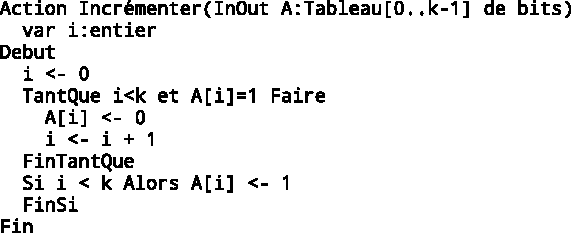
\includegraphics[width=180px]{Images/fig1.pdf}

\titre{Plan de cours}
\begin{enumerate}
	\item Introduction
	\item Concepts de base (objet, classe, envoi de message, hiérarchie)
	\item Illustrations et exemples (Java, Simula, SmallTalk
	\item Etude comparative de LO
	\item TP (Java, Eclipse)
\end{enumerate}

\titre{Histoire d'Ada}
Le département de la défense américain (Dod) est : 
\begin{itemize}
	\item Plus gros consommateur de logiciels
	\item 1968 - 73 : Le coût des SI augmente et le coût du matériel chute
	\item 73 : 7,5 milliards de dollars pour les Si
	\item 75 : 450 langages différents
	\item Réutilisabilité et partage de code inexistants
	\item 1983 : naissance d'Ada en réponse à la crise du logiciel et pour résoudre les pbs liés au dev de gros logiciels
	\item non issu d'un projet académique ou de recherche interne
\end{itemize}
Idée : Un seul langage incorporant tous les bons concepts de GL.\\

\titre{Paradigmes de programmation}
\begin{itemize}
	\item impérative
	\item fonctionnelle
	\item logique
	\item objet
	\item par contraintes
\end{itemize}

\newpage

\titre{Les domaines révolutionnés par la POO}
\begin{itemize}
	\item Génie logiciel (analyse, conception, programmation)
	\item Bases de données
	\item Intelligence artificielle (représentation des connaissances, programmation par agents)
\end{itemize}

\titre{Quel objet ?}
\begin{itemize}
	\item Des problématiques différentes $\rightarrow$ Des approches objet différentes
	\item Une préoccupation commune (approche modulaire de la complexité)
\end{itemize}
Pour distinguer les approches différentes, on change le voc :
\begin{itemize}
	\item Génie Logiciel : Objet
	\item IA : Schéma
	\item Ingénierie collaborative : Agent
	\item Bases de données : RDF
\end{itemize}

\titre{Quels languages :}
\begin{itemize}
	\item Java sous éclipse principalement
	\item Simula
	\item SmallTalk
\end{itemize}


\fiche{Analyse des algos récursifs}
\titre{Fonction $f(X)$} : $\left\{ \begin{array}{l} 
	\mathrm{si} \; \alpha(X) \; \mathrm{alors} \; \mathrm{val} \\
	\mathrm{sinon} \; f(X') \end{array} \right.$ \\

\titre{Simplification :} Pour analyser le temps d'exécution d'une fonction récursive, on va essayer de résumer à l'aide d'un seul entier $n$ le contexte $X$ de façon à ce que $n$ (correspondant généralement à la taille associée au contexte) décroit à chaque appel de $f$. \\

\titre{Exemple 1 :} \\
\code{
	Fonction F(m : entier) : entier $\theta(1)$\\
	Debut\\
		Si m = 0 $\theta(1)$ alors retourner $\vide$ $\theta(1)$\\
		Sinon retourner m*F(m-1) $\theta(1) + T(m - 1)$\\
	Fin\\
}

En pire cas : 
\begin{itemize}
	\item $T(0) = \theta(1)$
	\item $T(n) = \theta(1) + T(n-1)$
	\item Suite arithmétique de premier terme 1 et de raison 1 donc $T(n) = \theta(n+1) = \theta(n)$
	\item Donc factorielle s'exécute en temps linéaire
\end{itemize}

\newpage

\titre{Exemple 2 :} \\
\code{
	Fonction Max(V:Tableau[] de Elem, a,b : entier) : Elem $\theta(1)$\\
	Debut\\
		Si a = b alors retourner V[a] $\theta(1)$\\
		Sinon retourner Max2(V[a],Max(V,a+1;b)) $\theta(1) + T(n-1)$\\
	Fin\\
}

En pire cas :
\begin{itemize}
	\item $n = b - a$ (car $b$ et $a$ désignent les indices du tableau entre lesquels on cherche le max)
	\item Question : cout du passage de paramètre (par adresse : constant, par valeur : $n$) 
	\item $T(0) = \theta(1)$
	\item $T(n) = \theta(1) + \theta(n-1)$
	\item Suite arithmétique de premier terme 1 et de raison 1 donc $T(n) = \theta(n+1) = \theta(n)$
	\item Donc Max s'exécute en temps linéaire
\end{itemize}

\titre{Exemple 3 :} Recherche dichotomique récursive \\
\code{
Fonction Dicho(V:Tab[]; a,b:entier; x: Elem) :booléen $\theta(1)$\\
Var m: entier\\
Debut \\
	Si a = b alors retourner (x=V[a]) $\theta(1)$\\
	Sinon \\
		m $\leftarrow$ $\frac{a + b}{2}$ \\
		Si x $\leq$ V[m] alors retourner Dicho(V,a,m,x) $T(\frac{n}{2})$\\
		Sinon retourner Dicho(V,m+1,b,x) $T(\frac{n}{2})$\\
		FinSi\\
	FinSi\\
Fin\\
}

En pire cas :
\begin{itemize}
	\item $n = b-a$
	\item $T(0) = \theta(1)$
	\item $T(n) = \theta(1) + T(\frac{n}{2})$
	\item Donc $T(n) = \theta(\ln n)$
\end{itemize}

\titre{Exemple 4 :} Fibonacci \\
\code{
Foncion Fib(m:entier) :entier \\
Debut\\
	Si m = 0 alors retourner 0 \\
	Sinon si m = 1 alors retourner 1 \\
	Sinon retourner Fib(m - 1) + Fib(m - 2) \\
	Fin Si\\
Fin\\
}

En pire cas :
\begin{itemize}
	\item Le nombre d'appels à Fib est exactement le résultat Fib(m) + ou - 1
	\item Avec utilisation de l'exemple : Fib(m) $<<$ Myst(m)
	\item $T(0) = T(1) = \theta(1)$
	\item $T(n) = \theta(1) + T(n-1) + T(n-2)$
	\item Or Fib(n)/Fib(n-1) tend vers le nombre d'or $\phi$
\end{itemize}

\titre{Exemple intermédiaire :}
\code{
Fonction myst(m:entier):entier \\
Debut \\
	Si m = 0 retourner 1\\
	Sinon retourner myst(m-1) + myst(m-1) \\
	FinSi \\
Fin\\
}

\begin{itemize}
	\item $T(0) = \theta(1)$ 
	\item $T(n) = \theta(1) + 2T(n-1)$
	\item $T(n) = 1 + 2 + 2^2 + \ldots + 2^n = 2^{n+1} - 1 = \theta(2^n)$
\end{itemize}






\fiche{Analyse des récurrences linéaires}
\titre{Récurrence linéaire :} $$T(n+ p + 1) = f(n) + \displaystyle{\sum_{k=0}^{p}} a_kT(n+k)$$
	$$T(n+1) = aT(n) + 1$$
	$$T(n+2) = aT(n+1) + bT(n) + 1$$ \\

\titre{Résolution du cas d'ordre 1 :} \\

	$T(n) = \left\{ \begin{array}{c}
		n + 1 = \theta(n)\; \mathrm{si} \; a = 1 \\
		\frac{a^{n+1} - 1}{a - 1} = \theta(a^n) \\
	\end{array} \right.$ \\

\titre{Exemple 5 :} Hanoï \\
\code{
Fonction Hanoi(n,i,j,k)\\
Debut \\
	Si n > 0 alors \\
		Hanoi(n-1,i,j,k) \\
		Affiche("Je déplace de i vers j")\\
		Hanoi(n-1,k,j,i) \\
	FinSi \\
Fin \\
}

Temps de calcul :
\begin{itemize}
	\item $T(0) = \theta(1)$
	\item $T(n) = \theta(1) + 2T(n-1)$
	\item Donc $T(n) = \theta(2^n)$
\end{itemize}

\titre{Résolution du cas d'ordre 2 :} On simplifie le problème en faisant abstraction du 1 : On considère $T(n+2) = aT(n+1) + bT(n)$ ie $T(n+2) - aT(n+1) - bT(n) = 0$. \\
On pose $P(X) = X' - aX - b$. Il a deux racines $r_1$ et $r_2$ et la solution s'écrit sous la forme $\alpha r_1^n + \beta r_2^n$ (il suffit de le vérifier). \\
$$T(n) = \theta(r_1^n)$$

\titre{Fin du cas d'ordre 2 :} Le 1 ajoute une fois Fibonacci à la fin, donc ne change pas le $\theta$ \\

\titre{Fin de l'exemple 4 :} Fibonacci 
\begin{itemize}
	\item $P(X) = X^2 - X - 1$ donc $r_1 = \frac{1 + \sqrt{5}}{2} = \phi$ et $r_2 = \frac{1 - \sqrt{5}}{2}$ donc $r_2^n$ tend vers 0.
	\item $T(n) = \theta(\phi^n)$
\end{itemize}

\titre{Exemple 6 :} \\
\code{
Fonction Dummy(n:entier) :entier \\
	Si n $\leq$ 3 retourner 1 \\
	Sinon retourner Dummy(n-2) + Dummy(n-4) \\
	Fin Si \\
Fin \\
}

Solution :
\begin{itemize} 
	\item Le polynome est de la forme $X^4 - X^2 - 1$
\end{itemize}


\fiche{Analyse des diviser pour mieux régner}
\titre{Complexité des algos "diviser pour régner" :} Cas $T(n) = aT(\frac{n}{b}) + f(n)$ avec $a \geq 1$ , $b > 1$ et $T(0) = \theta(1) (=1)$ (on peut remplacer $\frac{n}{b}$ par sa partie entière inférieure ou supérieure) \\

\titre{Propriété :} 
\begin{itemize}
	\item Si $f(n) = O(n^{\mathrm{log}_ba-\varepsilon})$ ($\varepsilon > 0)$ alors $T(n)\in \theta(n^{\mathrm{log}_ba})$
	\item Si $f(n) = \theta(n^{\mathrm{log}_ba})$ alors $T(n) = \theta(n^{\mathrm{log}_ba}\ln n)$
	\item Si $f(n) = \Omega(n^{\mathrm{log}_ba+\varepsilon})$ ($\varepsilon > 0$) et $af(\frac{n}{b}) \geq cf(n)$ pour $n$ assez grand et $c$ une constante $< 1$. Alors $T(n) \in \theta(f(n))$
\end{itemize}

\titre{Exemple 7 :} La recherche dichotomique
\begin{itemize}
	\item $T(n) = T(\frac{n}{2}) + 1$ 
	\item On est dans le deuxième cas, donc $T(n) = \theta(\ln n)$
\end{itemize}

\titre{Exemple 8 :} Tri fusion \\
\code{
Fonction TriFusion(V:Tab,n:entier)\\
Var $n_1,n_2$ : entier \\
Var $V_1,V_2$ : Tab \\
Debut \\
	Si $n \geq 2$ Alors \\
		Diviser$(V,n,V_1,n_1,V_2,n_2)$ ($\theta(n)$)\\
		TriFusion$(V_1,n_1)$\\
		TriFusion$(V_2,n_2)$\\
		Fusionner$(V_1,n_1,V_2,n_2,V)$ ($\theta(n)$)\\
	FinSi\\
Fin \\
}

Temps d'exécution :
\begin{itemize}
	\item $T(n) = 2T(\frac{n}{2}) + \theta(n)$
	\item $f(n) = \theta(n)$ donc on est dans le deuxième cas
	\item $T(n) = \theta(n\ln n)$
\end{itemize}


\fiche{TD}
\titre{Question 1}\\
\\
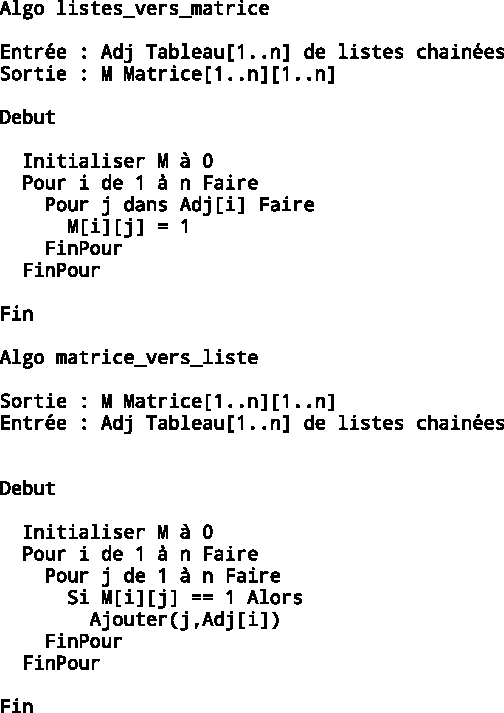
\includegraphics{Images/fig19.pdf}
\\
\newpage
\titre{Question 2}\\
\\
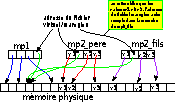
\includegraphics[width=200px]{Images/fig20.pdf}
\\
\\
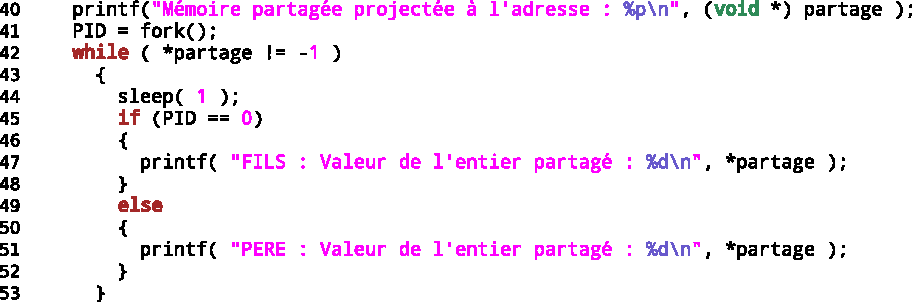
\includegraphics[width=300px]{Images/fig21.pdf}
\\
\titre{Question 3}
\begin{enumerate}
	\item $K_n$ possède $\frac{n(n-1)}{2}$ arêtes.
	\item $\bar{K_n}$ possède 0 arête
	\item $O(n^2)$
\end{enumerate}

\titre{Question 4} Il y a deux sous graphes isomorphes à $K_3$ et aucun isomorphe à $\bar{K_3}$
\newpage
\titre{Question 5} \\
\\

\includegraphics[width=100px]{Images/fig23.pdf}
\\
\titre{Question 6} 
\begin{enumerate}
	\item .\\ 
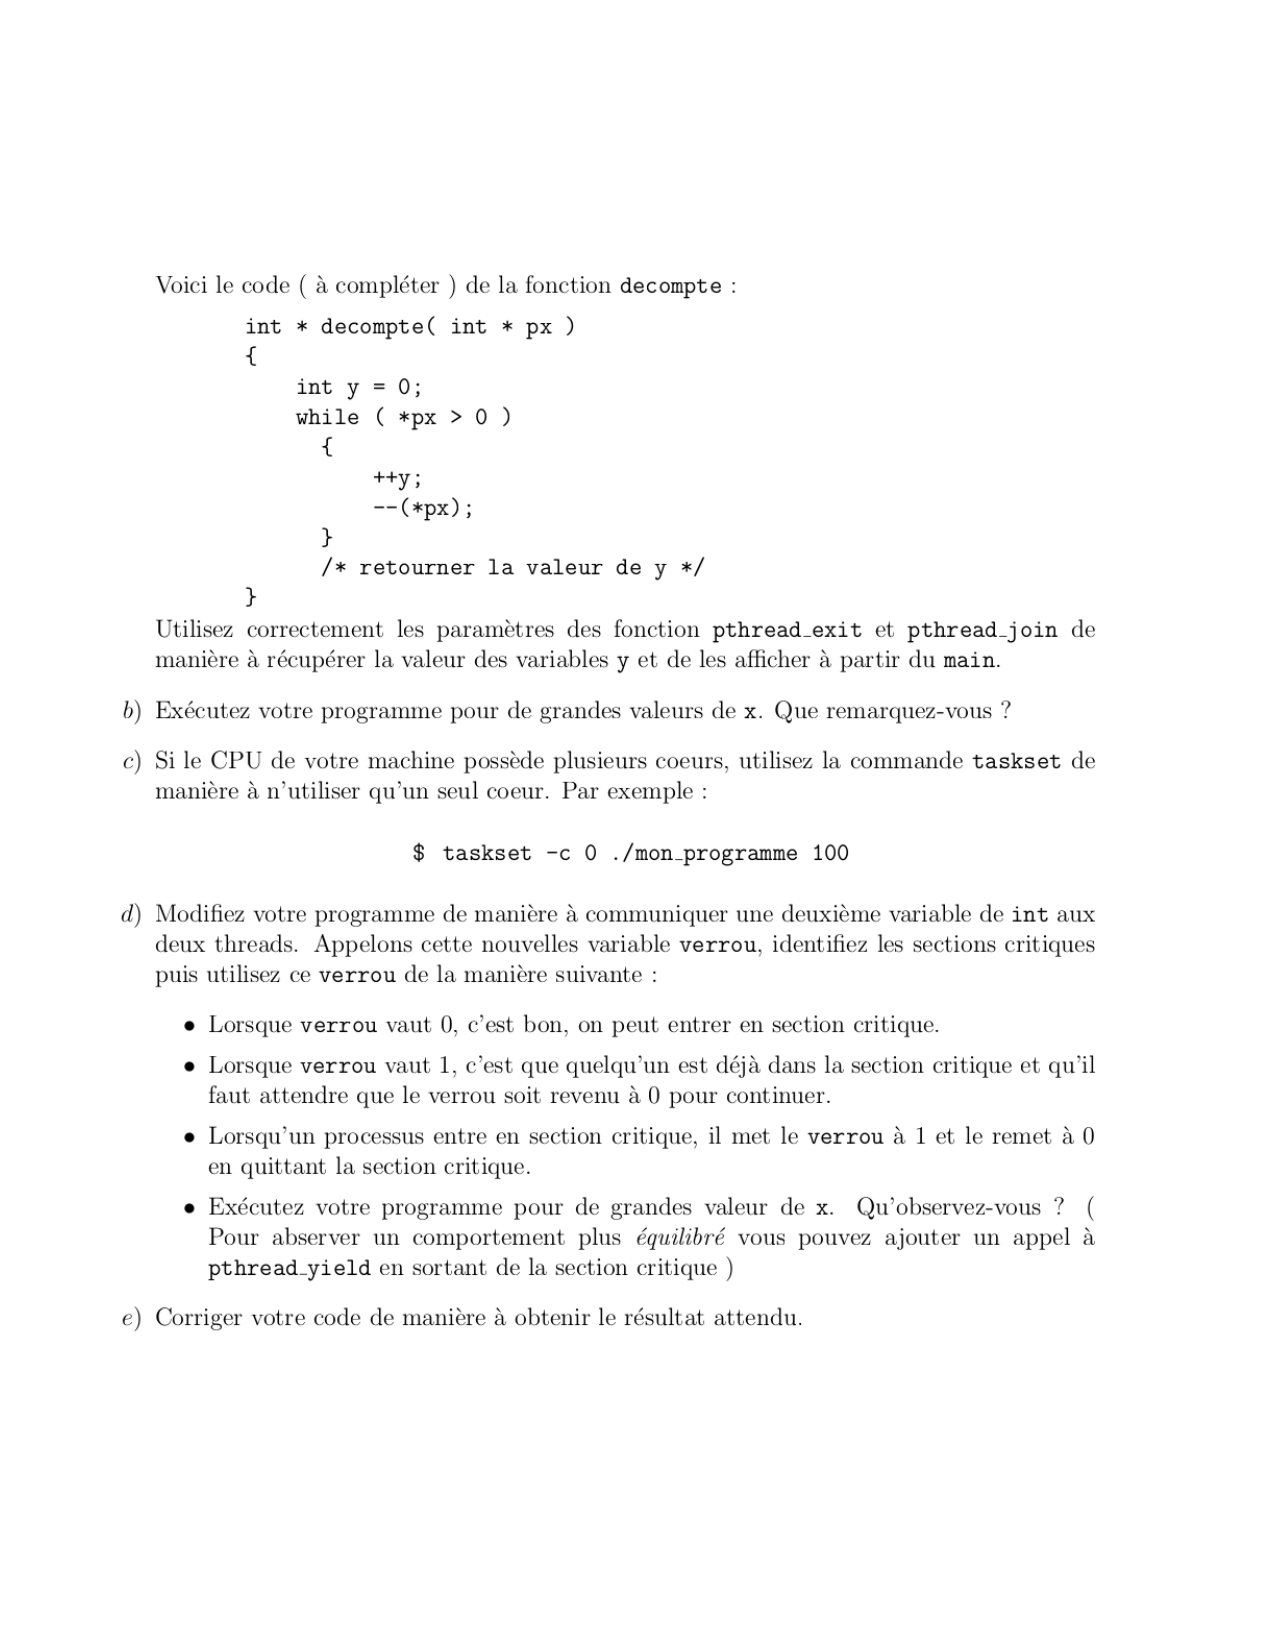
\includegraphics{Images/fig24.pdf}
	\item $O(n^2)$
	\item .\\
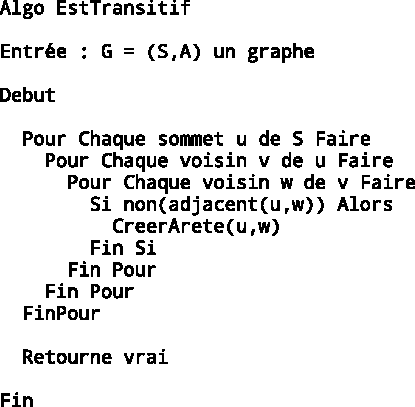
\includegraphics{Images/fig25.pdf}
	\item $O(n^2)$
	\item Faire mieux ???
\end{enumerate}

\titre{Question 7} Il faut commencer par enlever une allumette \\
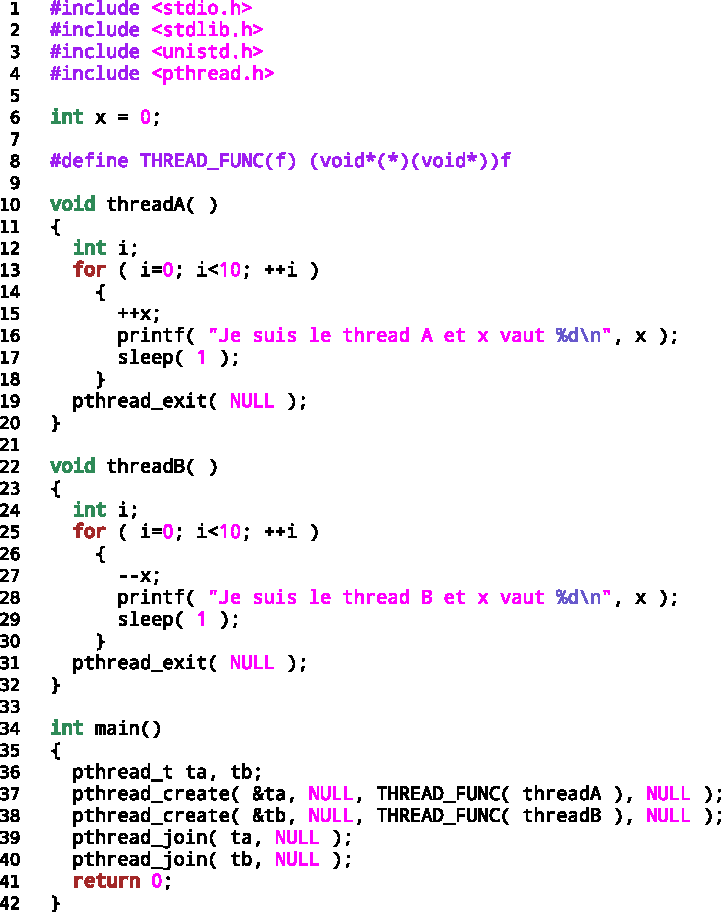
\includegraphics[width=250px]{Images/fig26.pdf} \\

\titre{Question 8} P = passeur, C = choux, B = chèvre (bêêê), L = loup \\
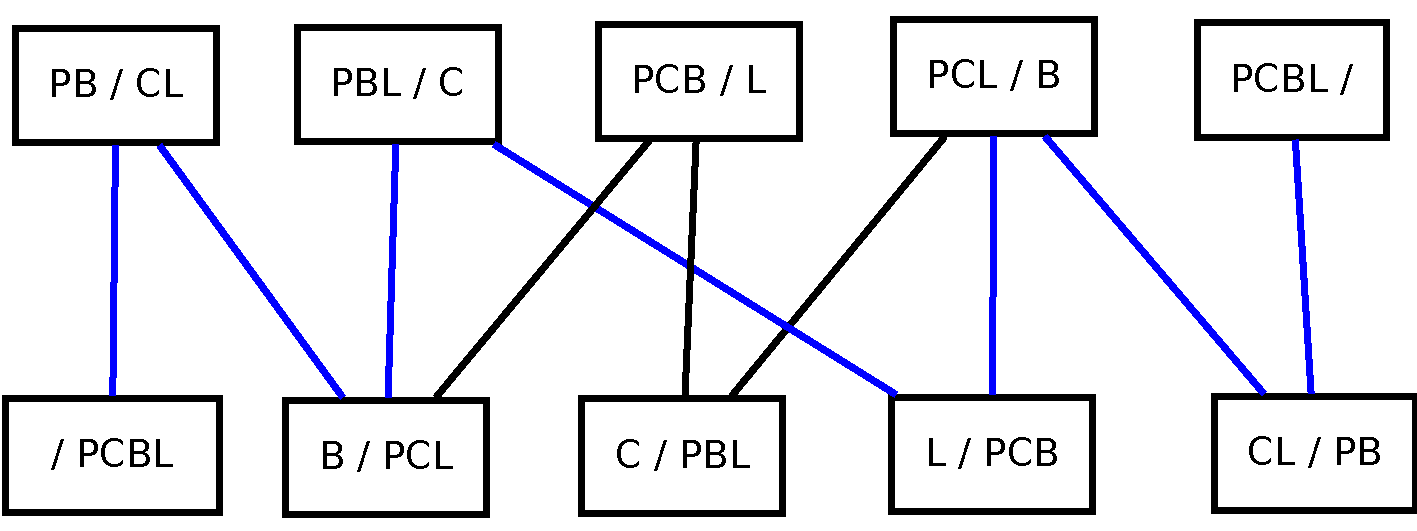
\includegraphics[width=250px]{Images/fig27.pdf} \\

\titre{Question 9} \\
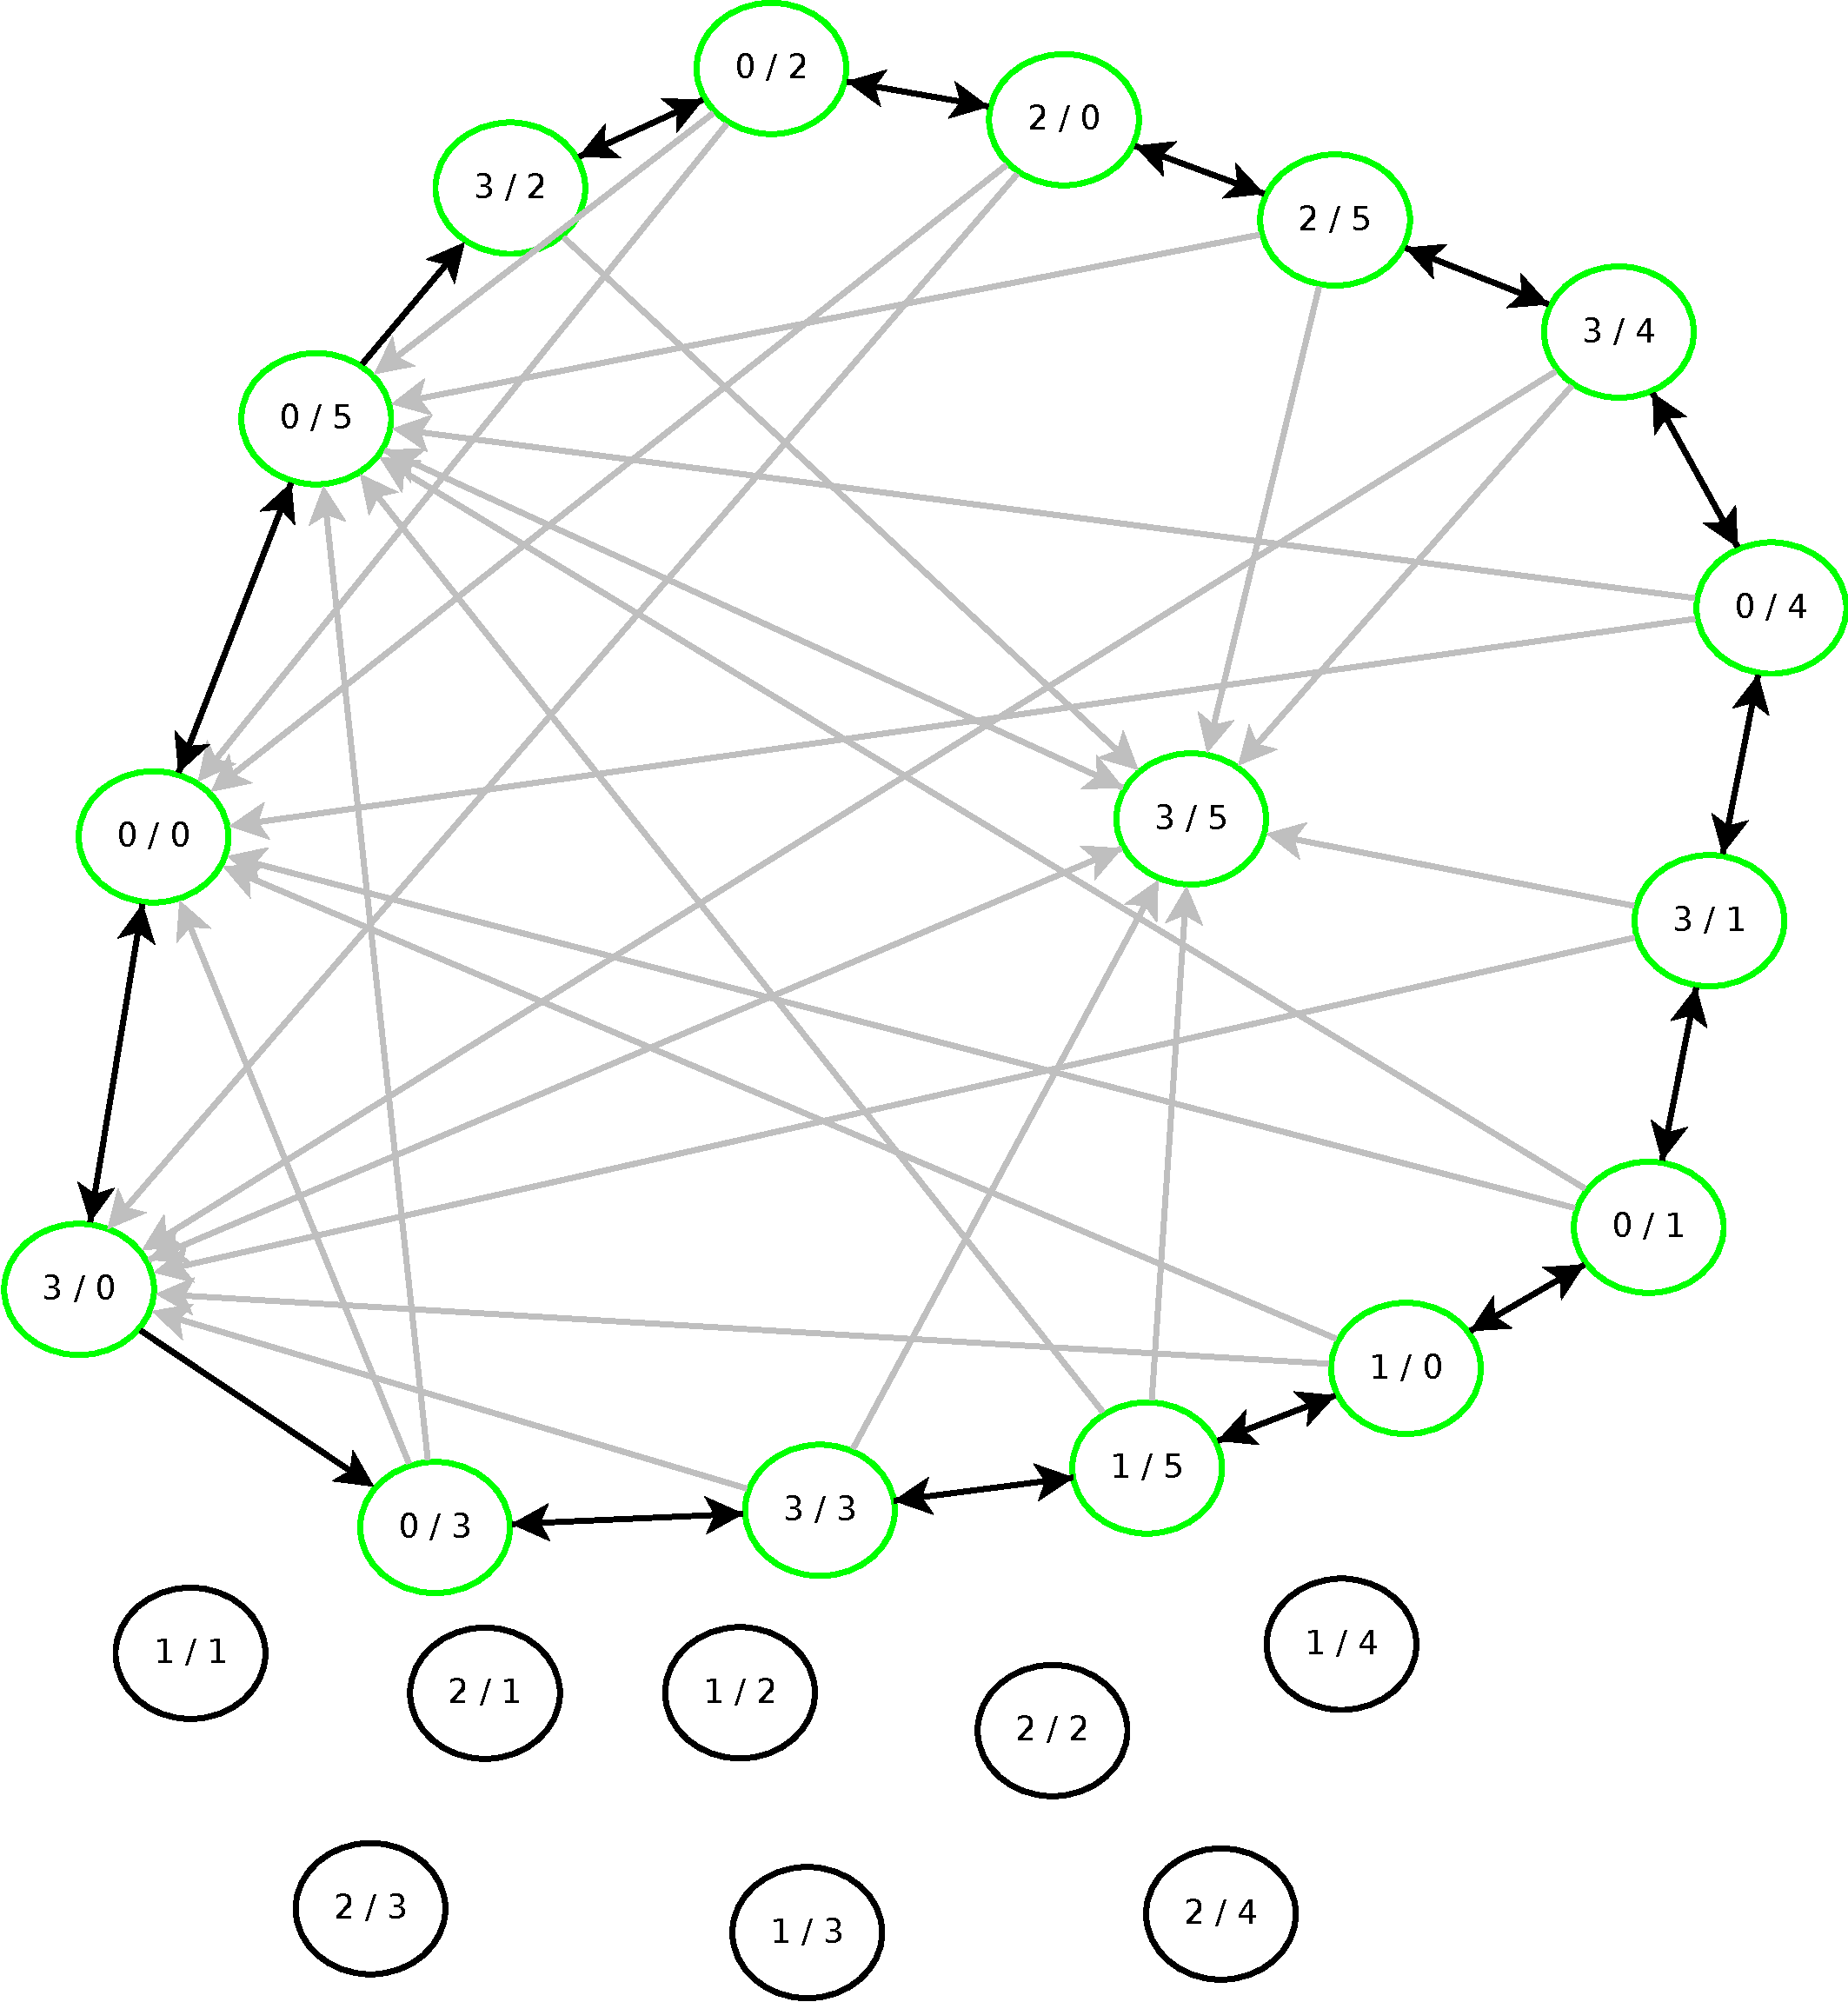
\includegraphics[width=300px]{Images/fig28.pdf} \\


\fiche{Analyse asymptotique expérimentale}
\titre{Principe :} On mesure de façon expérimentale le temps d'exécution de 2 programmes pour des valeurs de $n$ données, avec $T_1(n) = n^2$ et $T_2(n) = 1000n$ : 
$$\begin{array}{c|c|c|c|c|c|}
n	& 10 & 20 & 40 & 80 & 160 \\ \hline
T_1 & & & & & \\ \hline
T_2 & & & & & \\ \hline
\end{array}$$

\titre{Idée :} On va tracer les courbes dans un repère utilisant une échelle logarithmique. Alors la fonction $an^b$ devient $\log_2(a) + b\log_2(n)$ \\
Preuve : $\log(T(n)) = \log(an^b) = \log a + \log n^b = \log a + b\log(n)$ \\

\titre{Pour les complexités en $an^b\log(n)$ :} Poser $T_2(n) = \frac{T(n)}{n^b}$ et mettre l'échelle logarithmique sur l'axe des abscisses.


\fiche{Analyse amortie}
\titre{Principe :} Calculer le coût moyen de chaque opération dans le pire cas de séquence d'opérations. \\

\titre{3 techniques standard :}
\begin{itemize}
	\item Méthode par agrégat
	\item Méthode comptable
	\item Méthode du potentiel
\end{itemize}

\titre{Méthode par agrégat :} On montre que pour toute suite d'opérations, le temps total est $T(n)$ dans le pire cas et le cout amorti (= cout moyen) de chaque opération est $\frac{T(n)}{n}$. \\

\titre{Exemple : La pile } \\
On a 3 opérations sur les piles :
\begin{itemize}
	\item Empiler(S,x) $\theta(1)$
	\item Depiler(S) $\theta(1)$
	\item Multidepiler{S,k} $\theta(min(k,s))$ ($s=$Card$S$)
\end{itemize}
L'utilisateur faire une série de $n$ opérations parmi ces 3 là.
\begin{itemize}
	\item $n$ fois empiler,depiler $\theta(n)$
	\item $n$ Multidepiler Cout borné par les $k$ choisis et le nombre d'éléments de la pile
	\item $\frac{n}{2}$ empiler et $\frac{n}{2}$ multidépiler Donc $\frac{n}{2}\theta(n) = O(n^2)$
\end{itemize}
En réalité, on empile et dépile $n$ fois quoi qu'il arrive donc la complexité en pire cas est $\theta(n)$\\
Cout amorti de chaque opération = Cout total / $n$ = $\theta(1)$

\titre{Exemple : Le compteur de bits}\\
On a un tableau $A[0..k-1]$ de bits. Donc $A$ représente un entier $x=\displaystyle{\sum_{i=0}^kA[i]2^i}$ qu'on appelle le compteur.\\
On a l'opération incrémenter qui ajoute 1 à $x$ \\
\\
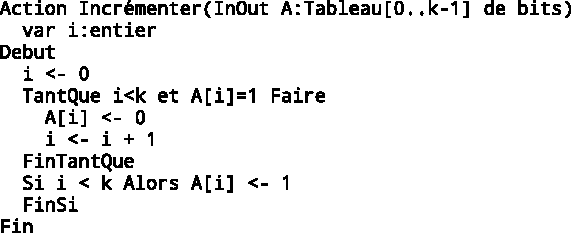
\includegraphics{Images/fig1.pdf}
\\
On compte le nombre de fois que chaque bit est modifié \\
Cout total = $n\displaystyle{\sum_{i=0}^{k'}}(\frac{1}{2})^{k'}$ avec $k'=\log_2 n$ donc Cout total $\leq 2n$ \\
Le cout amorti est donc $\theta(1)$



\fiche{TD}
\titre{Exercice 5 :} \\
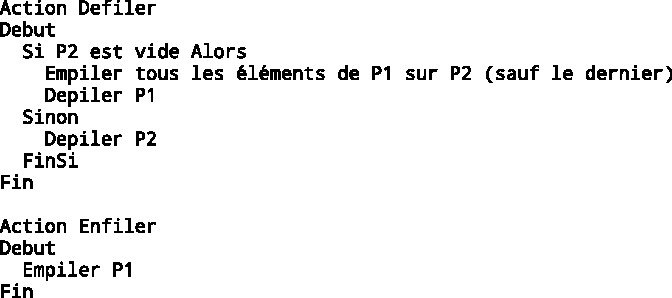
\includegraphics{Images/fig2.pdf} \\
On effectue $n$ opérations : $E$ l'ensemble des $e_i$ les enfilements, et $D$ l'ensemble de $d_i$ les défilements. \\
Cout total = $\sum e_i + \sum d_i$. \\
On a $\sum e_i \leq n$ car le cout d'un $e_i$ est 1. \\
Une fois qu'on a dépilé $P_1$ avec un cout égal à la taille de $P_1$, il se passe exactement taille de $P_1$ opérations avec un cout de 1, puis on recommence ce cycle. \\
$\sum d_i = tP1 + \sum_{k=1}^{tP1}1 + t'P1 + \sum_{k=1}^{t'P1}1 \ldots \leq 2n$ \\
Conclusion : Cout total $\leq 3n$. Donc Cout total est $O(n)$. \\
De plus, si on ne fait que des empilements le cout est $\theta(n)$. Donc Cout total est $\theta(n)$. \\
Donc le cout amorti est $\frac{\theta(n)}{n}=\theta(1)$


\fiche{Structures de données pour ensembles disjoints}
\titre{Définition :} On appelle ensembles disjoints une collection $S=S_1,\ldots,S_n$ d'ensembles deux à deux disjoints. On va effectuer des opérations sur ces ensembles (ex : union, déterminer si un élément est dans un des ensembles, si deux ensembles sont contenus dans un autre ensemble etc). \\

\titre{Utilisations classiques :}
\begin{itemize}
	\item Calculer les composantes connexes d'un graphe (fermeture transitive de la relation d'adjacence)
	\item Calculer des classes d'équivalence de façon générale
	\item Déterminer si un graphe contient un cycle (algo de Kruskal)
\end{itemize}

\titre{Opérations sur ces structures :} Les éléments des ensembles sont appelés "objets" (pointeur vers un élément avec des informations) :
\begin{itemize}
	\item Creer-ensemble(x:objet) : Créer un ensemble réduit au singleton x
	\item Trouver-ensemble(x:objet) : retourne un objet qui est le représentant de tous les objets du meme ensemble.
	\item Union(x,y:objet) avec x $\neq$ y et Trouver-ensemble(x) $\neq$ Trouver-ensemble(y). Attribue un nouveau représentant et réalise l'union.
	\item On pourrait rejouter des opérations de division d'ensemble mais ça ne présente aucune difficulté.
\end{itemize}

\titre{Exemple :} Calcul de composantes connexes. On voudrait savoir si deux sommets d'un graphe sont dans la même composante connexe (ie existe-t-il un chemin entre ces deux sommets), combien il y a de composantes connexes dans le graphe, etc. \\

\includegraphics{Images/fig3.pdf} \\
Le cout est donc n Creer-ensemble + 2m Trouver-ensemble + min(n,m) Unions \\

\titre{Représentation par listes chaînées :} On représente chaque ensemble par une liste chainée enrichie. 
\begin{itemize}
	\item Creer-ensemble est en $\theta(1)$
	\item Trouver-ensemble est en $\theta(1)$
	\item Union : pour pouvoir fusionner la plus petite à la grande, il nous faut rajouter une donnée : le nombre d'éléments de chaque liste. Cela permet de réduire la complexité au point où $n$ creer-ensemble et $m$ opérations quelconques, alors le coût amorti total est de $\theta(m+n\mathrm{ln}n)$ On le démontre avec la méthode des agrégats. 
\end{itemize}

\titre{Preuve :} \\
La complexité totale correspond au nombre de fois où le lien "représentant" est modifié. \\
Pour un objet x, son représentant est modifié lors d'une union où x était dans le plus petit ensemble. \\
Au début, x est dans un ensemble à un élément. \\
Si son représentant est modifié une fois alors il est dans un ensemble à au moins 2 éléments.\\
Si son représentant est modifié une deuxième fois alors il est dans un ensemble à au moins 4 éléments.\\
La taille double à chaque fois, d'où le $\mathrm{ln}n$ \\
Et il y a n éléments, donc on a au maximum $n\mathrm{ln}n$ changements de représentants.\\

\titre{Représentation par forêt :} Un ensemble a un représentant unique qui va être la racine d'un arbre. Tous les éléments d'un ensemble vont être dans le même arbre, et on a un arbre par ensemble. La forêt est l'union disjointe des arbres. Chaque élément, en plus de sa valeur, stockera un pointeur vers son père dans l'arbre (ou lui même si c'est la racine), ainsi qu'u entier appelé rang. \\

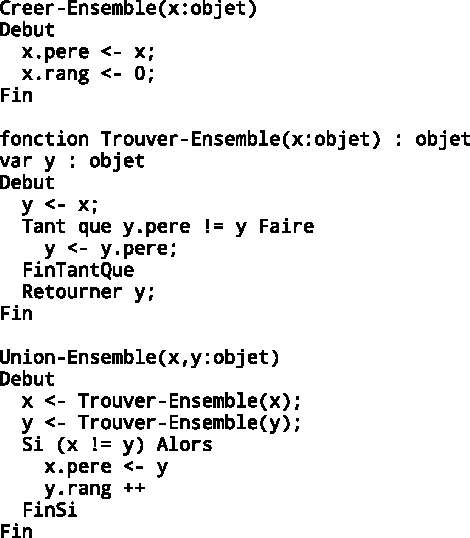
\includegraphics{Images/fig4.pdf}\\

\titre{Idées :}
\begin{itemize}
	\item Union par rang : on connecte l'arbre qui a le plus petit rang à l'autre. \\
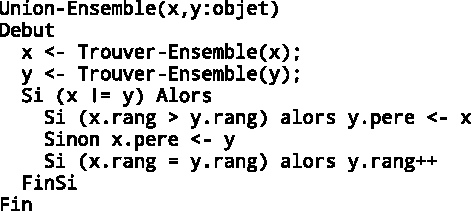
\includegraphics{Images/fig5.pdf}\\
	\item Compression de chemin : On profite d'un appel à Trouver-Ensemble pour mettre à jour tous les pères sur le chemin de l'objet jusqu'à sa racine.\\
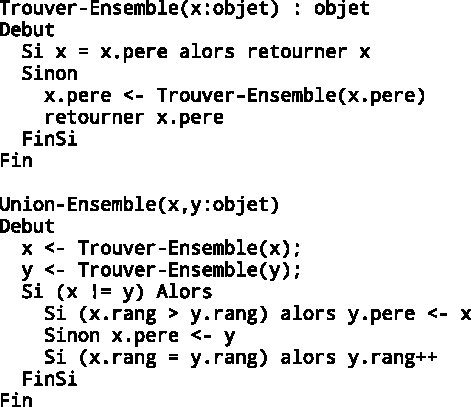
\includegraphics{Images/fig6.pdf}\\
\end{itemize}

\titre{Théorème de Tarjan (1975) :} Si on utilise ce type de structure Union-Find avec union par rang et compression de chemin, alors une séquence arbitraire de m opérations Creer-Ensemble, Trouver-Ensemble et Union-Ensemble prend un temps en $\theta(m\alpha(n))$ où $\alpha(n)$ croit très lentement (impossible de représenter en mémoire un entier $n$ qui rend $\alpha(n) \leq 4$). \\

\titre{Explication :} $\alpha$ est l'inverse d'une fonction qui croit très vite : $A_k(1)$ ... $\alpha(n)$ = plus petit $k$ tel que $A_k(1)\geq n$. Avec $A_k$ la fonction de Ackermann : qui à $k\geq 0, j \geq 1$ associe $A_k(j) = \left\{ \begin{array}{l}
	j+1 \mathrm{si} k = 0
	A_{k-1}(A_{k-1}( \ldots A_{k-1}(j)))) \mathrm{sinon} \end{array} \right.$

$$
\begin{array}{c|cccccc}
	j & 1 & 2 & 3 & 4 & 5 & 6 \\ \hline
A_0(j) & 2 & 3 & 4 & 5 & 6 & 7  \\ \hline
A_1(j) & 3 & 5 & 7 & 9 & 1 & 13  \\ \hline
A_2(j) & 7 & 23 & 63 & \ldots \\ \hline
A_3(j) & 2047 & >2^{2^{27}} & \ldots \\ \hline
A_4(j) & >> 2^{2048} & \ldots \\ \hline
\end{array}
$$

\titre{Conclusion :} Union-Find peut être considéré comme linéaire.\\

\titre{Exercice :} Quel est le rang max que l'on peut obtenir avec 7 unions sur 8 éléments ? Réponse : 3 (en réalité pour faire un rang $k$ il faut $2^k$ éléments. On voit donc qu'il y a majoration par $m\ln n$. \\

\titre{Exercice :} Si on fait trouver-Ensemble sur un sommet de profondeur $k$, quelle est la variation de la somme des profondeurs de l'arbre ? \\



\fiche{TD}
\input{Includes/10_TD3.tex}

\fiche{Géométrie algorithmique}
\titre{Objectif :} Etudier les algortithmes pour résoudre des problèmes géométriques. \\

\titre{Applications :}
\begin{enumerate}
	\item CAO
	\item Jeux vidéos en 2D et 3D
	\item Résistance des matériaux
	\item Robotique
	\item Réseaux
\end{enumerate}

\titre{Géométrie euclidienne :} Points et vecteurs du plan ou de l'espace. Cela suppose qu'on dispose d'un type nombre réel (problème : sensibilité aux perturbations). \\

\titre{Solutions à ces problèmes :}
\begin{enumerate}
	\item Méthodes algébriques
	\item Utiliser des opérations "pas dangereuses" (addition, soustraction), pour la multiplication il faut une précision doublée, la division est dangereuse
	\item Utiliser des nombres à précision arbitraire (fonctionne mais ralentit le code d'un facteur 100 à 200)
	\item Utiliser seulement le signe plutôt que la valeur
	\item Ne faire des calculs qu'en cas de "doute" (calcul paresseux)
	\item Tout faire avec des entiers (géométrie discrète)
\end{enumerate}
Il existe des bibliothèques standard pour faire ça (ex : CGal en C++)\\
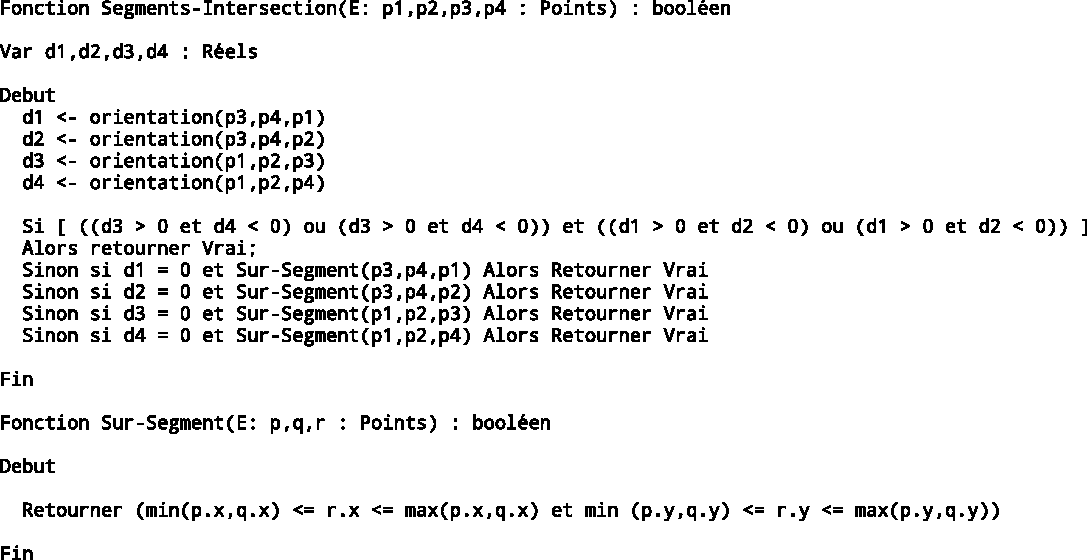
\includegraphics{Images/fig7.pdf}

\titre{Définition des éléments de base dans le plan :}
\begin{enumerate}
\item typedef struct { double x; double y; } Point; 
\item typedef struct { Point O; Point E; } Segment; C'est l'ensemble des points entre O et E $\rightarrow$ comment faire ça précisément ? On utilise les combinaisons linéaires sur O et E : $P = \alpha O + (1 - \alpha) E$ avec $\alpha \in [0;1]$ ie $[OE]=\{ \alpha O + (1 - \alpha) E \tq \alpha \in [0;1] \}$ cet ensemble est appelé ensemble des combinaisons convexes.
\item Longueur du segment $[OE]$ = distance euclidienne entre $O$ et $E$ = norme de $\vec{OE}$ = $\sqrt{(E.x - O.x)^2 - (E.y - O.y)^2}$. En géométrie algorithmique, on privilégie la distance au carrée (pour les erreurs et le temps de calcul).
\end{enumerate}

\titre{Question typique :} Etant donné un point $P$ et une droite $(P_1P_2)$, le point est il sur la droite, à sa gauche et à sa droite ? On utilise le déterminant de $\vec{P_1P_2},\vec{P_1P}$ (positif : $P$ est à gauche, négatif : $P$ est à droite, nul : $P$ est sur la droite.) Cela s'appelle la fonction d'orientation : retourne $(P_2.x - P_1.x)(P_2.y - P_1.y) - (P_2.y - P_1.y)(P.x - P_1.x)$\\

\titre{Question :} Comment déterminer si deux segments consécutifs $[P_1P_2]$ et $[P_2P_3]$ forment un vira	ge à droite ? Réponse on regarde si Orientation($P_1,P_2,P_3$) est négatif. \\

\titre{Question :} Comment déterminer si deux segments sont sécants ? $[P_1P_2]$ et $[P_3P_4]$ s'intersectent si $P_1$ et $P_2$ ne sont pas du même côté de $[P_3P_4]$ et que $P_3$ et $P_4$ ne sont pas du même côté de $[P_1P_2]$\\

\titre{Polygone :} Courbe du plan refermée sur elle même, composée d'une suite de segments de droite consécutifs appelés les côtés du polygone. Un sommet est l'intersection de 2 côtés consécutifs, et le nombre de sommets est égal au nombre de côtés.\\

\titre{Polygone simple :} Seuls les segments consécutifs s'intersectent en leurs extrémités.\\

\titre{Structure de données :} On caractérise un polygone par la séquence de ses sommets (modulo un choix de sommet de départ arbitraire)\\

\titre{Propriété :} Si un polygone est simple, alors il découpe le plan en deux zones connexes : l'intérieur et l'extérieure.\\

\titre{Exercice :} Ecrire un algorithme de complexité en $O(n^2)$ qui décide si un polygone donné sous forme de tableau est simple. ($n=$ nombre de côtés).\\
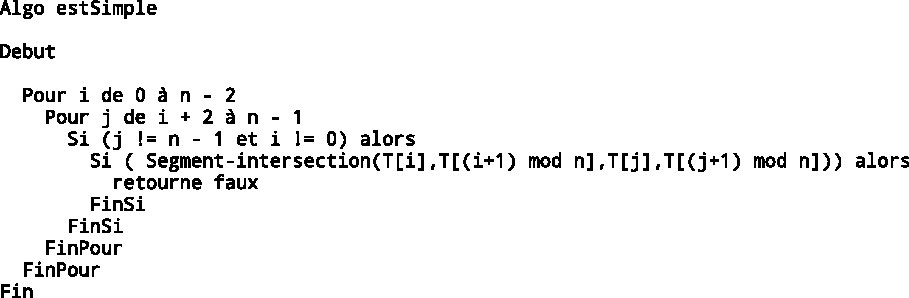
\includegraphics{Images/fig8.pdf}\\

\titre{Question :} Complexité minimale pour déterminer la liste des points d'intersections d'un polygone ($\Omega (n^2)$) (cf polygone type grille). \\

\titre{Complexité minimale pour décider si un polygone est simple :} $\theta(n\ln n)$ (algo pour tester si il y a une intersection au sein d'un ensemble quelconque de segments adapté au cas des polygones). \\

\titre{Algorithme par balayage d'une droite :} On se donne une direction de calcul (l'axe des abscisses), et on fait "avancer un droite virtuelle" (perpendiculaire à l'axe des ordonnées) \\
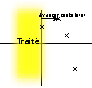
\includegraphics[width=150px]{Images/fig9.pdf} \\
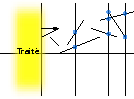
\includegraphics[width=150px]{Images/fig10.pdf} \\

\includegraphics{Images/fig11.pdf} \\

\titre{Question :} Etant donné un point x, est-ce que x est à l'intérieur d'un polygone simple ? Astuce depuis x on trace un rayon vers l'infini et on compte les intersections avec le bord (si je pars de l'intérieur c'est impair, sinon c'est pair) \\
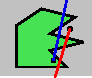
\includegraphics[width=150px]{Images/fig12.pdf} \\

\titre{Convexité :} Une partie $C$ du plan est convexe si et seulement si $\forall x,y \in C$ le segment $[xy]$ est inclus dans $C$. (exemple : algo GJK pour la détection de collisions)\\

\titre{Utilisation :} A partir d'une forme non convexe, on cherchera son enveloppe convexe. \\

\titre{Remarque :} Si $P$ est un ensemble de points ou un polygone, alors le contour de $\mathrm{Conv}(P)$ est un polygone simple. \\

\titre{Propriété :} Dans un polygone simple convexe, deux côtés consécutifs font toujours un "virage à gauche". \\

\titre{Propriété :} Si $P_iP_{i+1}$ est un côté de l'enveloppe convexe des points $(P_i)_{i\in\{0,\ldots,n-1\}}$, alors tous les autres points dont du côté gauche.\\

\titre{Algo naïf de calcul de l'enveloppe convexe :}

\end{document}
